% -------------------------------------------------------------------------------------------------------
%-----------------------------CONSULTA DE RECURSOS HUMANOS---------------------------------
% -------------------------------------------------------------------------------------------------------

\chapter{Gestión de Recursos Humanos}
    \section{Consulta de Recursos Humanos}
        Cuando el Jefe de Innovación Educativa da clic en la sección de \textbf{Gestionar Recursos Humanos} aparecerá la siguiente pantalla:
        
        % Imagen menu
        
        \begin{figure}[!hbtp]
        	\centering
        	\hypertarget{consultarrh}{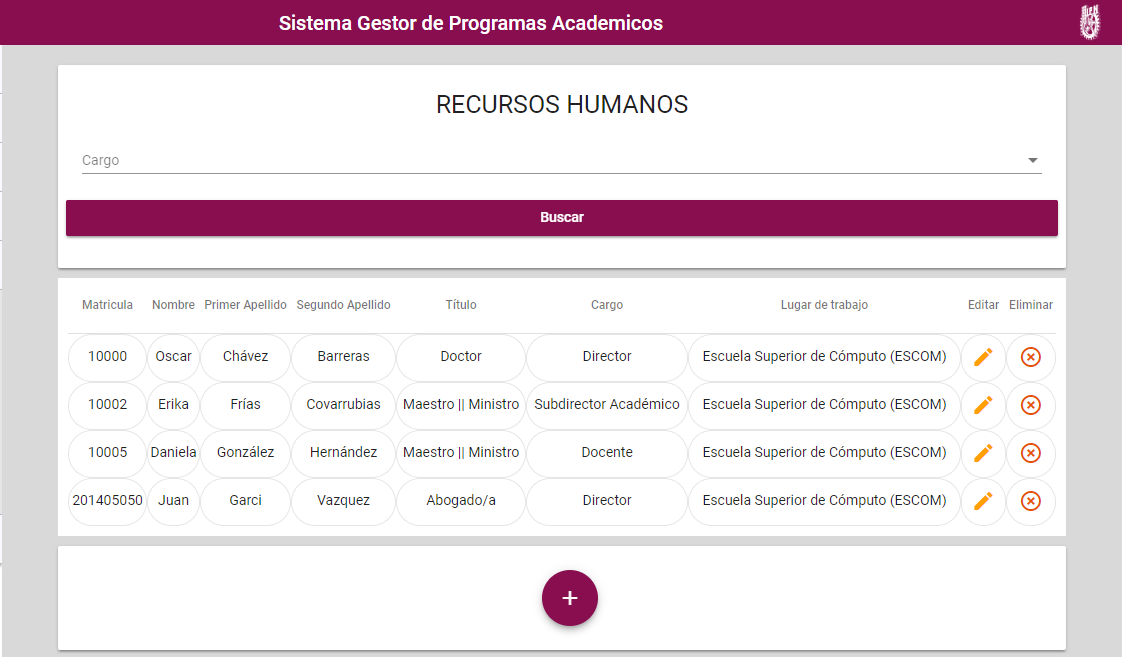
\includegraphics[width=0.7\linewidth]{images/SP1/ConsultarRH}}
        	\caption{Pantalla para consultar Recursos Humanos}
        	\label{consultarrh}
        \end{figure}

        En donde aparecerá, de forma predeterminada, todos los Recursos Humanos a su cargo registrados en el sistema al momento. Tendrá a su disposición tres funciones:

    	\subsection{Buscar Recursos Humanos según su cargo}
        
        	Para ello, el Jefe de Innovación Educativa tendrá que seleccionar el cargo que desea consultar en el siguiente componente:
        
        	\begin{figure}[!hbtp]
        		\centering
        		\hypertarget{cargo1}{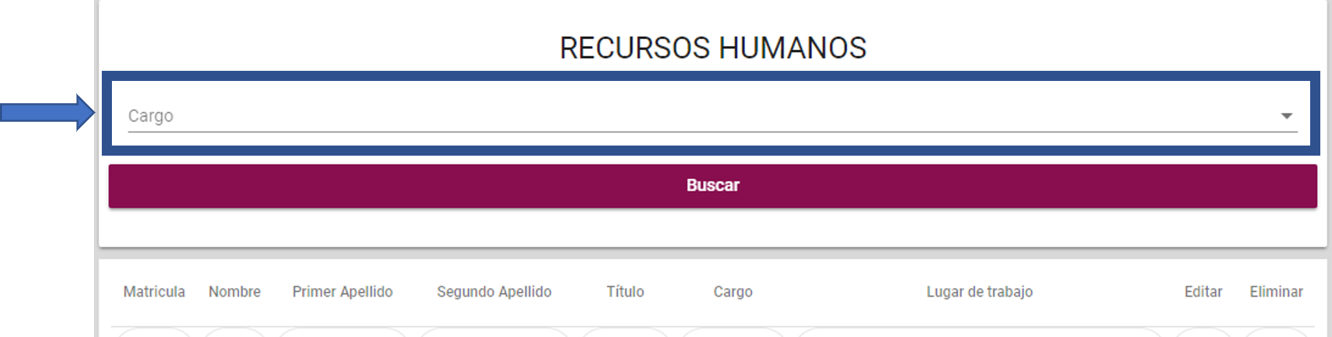
\includegraphics[width=0.7\linewidth]{images/SP1/BtnCargo1}}
        		\caption{Selección de Cargo}
        		\label{cargo1}
        	\end{figure}

        	\begin{figure}[!hbtp]
        		\centering
        		\hypertarget{cargo}{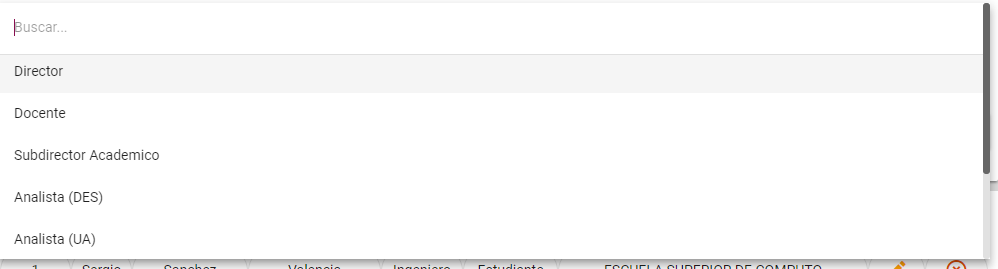
\includegraphics[width=0.7\linewidth]{images/SP1/BtnCargo}}
        		\caption{Despliegue de cargos}
        		\label{cargo}
        	\end{figure}
        
        	Luego, deberá de dar clic en el botón \IUbutton{Buscar}, y a continuación el sistema mostrará todos los Recursos Humanos que tengan el cargo seleccionado.
        	\begin{figure}[!hbtp]
        		\centering
        		\hypertarget{buscar}{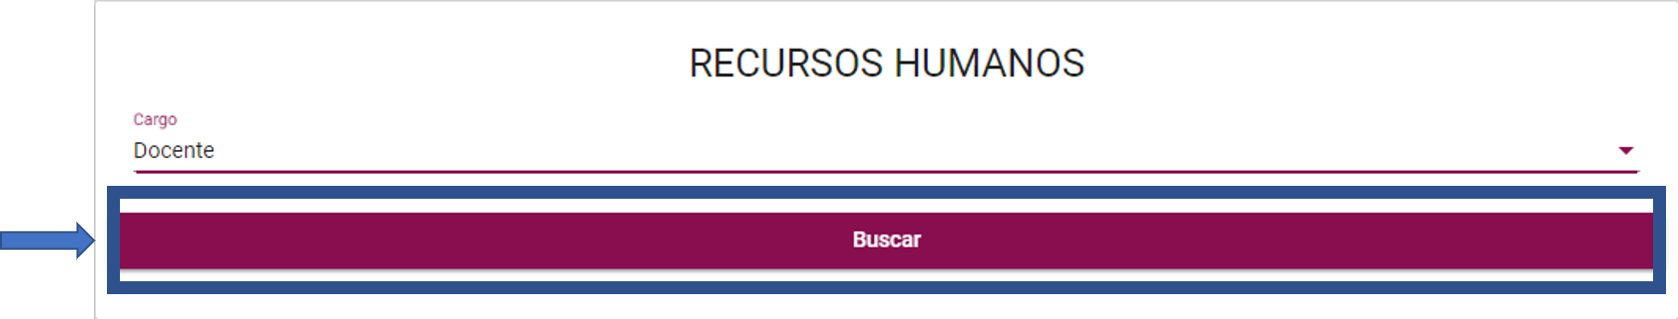
\includegraphics[width=0.7\linewidth]{images/SP1/BtnBuscar2}}
        		\caption{Botón Buscar Recursos Humanos}
        		\label{buscar}
        	\end{figure}

	    \subsection{Editar Recursos Humanos}

        	Para ello, el Jefe de Innovación Educativa tendrá que dar clic en el botón con el icono de un lapiz amarillo que esta al lado del Recurso Humano que desea modificar. Al hacer esto, el sistema redireccionará al usuario a la pantalla de \hyperlink{editarrh}{\textit{Editar Recurso Humano}}.
        
        	\begin{figure}[!hbtp]
        		\centering
        		\hypertarget{editar}{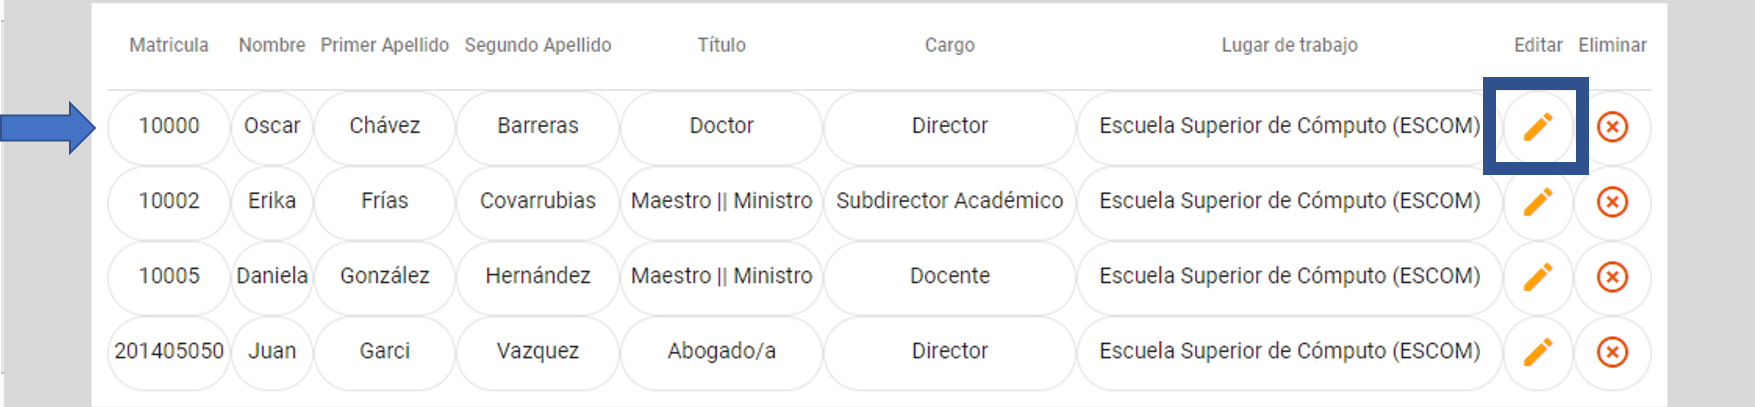
\includegraphics[width=0.7\linewidth]{images/SP1/BtnEditar}}
        		\caption{Botón Editar Recursos Humanos}
        		\label{editar}
        	\end{figure}
    \newpage
	    
	    \subsection{Eliminar Recursos Humanos}

        	Para ello, el Jefe de Innovación Educativa tendrá que dar clic en el botón con el icono de una cruz roja que esta al lado del Recurso Humano que desea eliminar. 

        	\begin{figure}[!hbtp]
        		\centering
        		\hypertarget{eliminar}{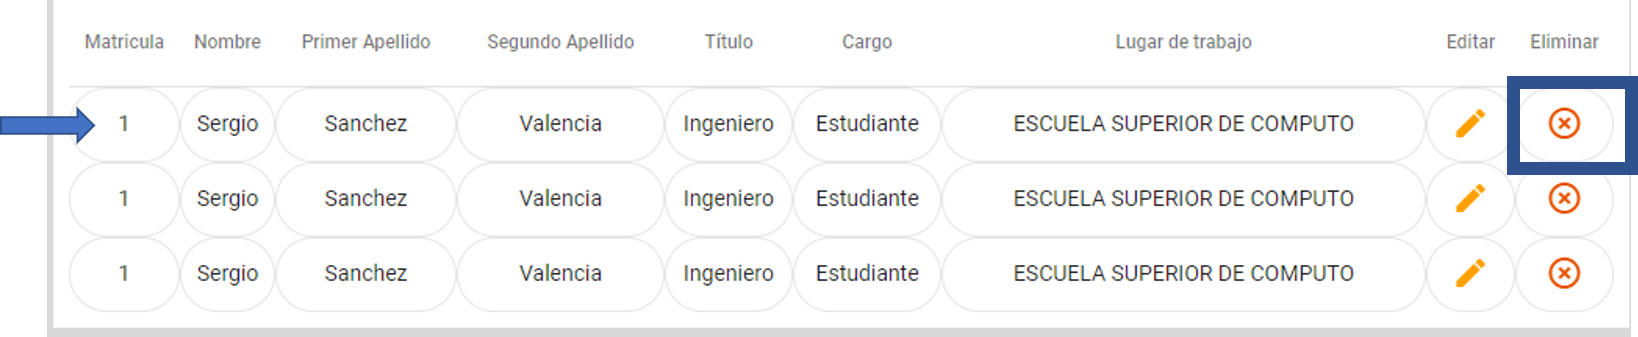
\includegraphics[width=0.7\linewidth]{images/SP1/BtnEliminar}}
        		\caption{Botón Eliminar Recursos Humanos}
        		\label{eliminar}
        	\end{figure}
        
        	Al hacer esto, el sistema despliegará el siguiente mensaje:
        	%Imagen del MSG34
        
        	Para confirmar, el usuario debe dar clic en el botón \IUbutton{Sí}, y el Recurso Humano será removido del sistema (ya no será desplegado en ninguna pantalla).\\
        
        	Para cancelar, el usuario debe dar clic en botón \IUbutton{No}, el mensaje se cerrará y regresaremos a la pantalla de \hyperlink{consultarrh}{\textit{Consultar Recursos Humanos}}.\\

    	\subsection{Registrar Recursos Humanos}

        	Para ello, el Jefe de Innovación Educativa tendrá que dar clic en el botón \IUbutton{+} en la parte inferior de la pantalla.
        
        	\begin{figure}[!hbtp]
        		\centering
        		\hypertarget{add}{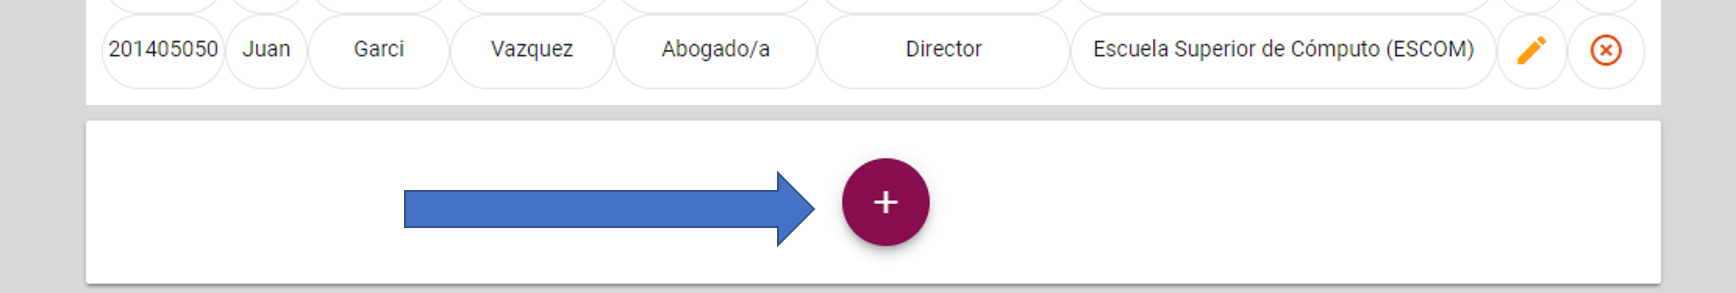
\includegraphics[width=0.7\linewidth]{images/SP1/BtnAgregar}}
        		\caption{Botón Agregar Recursos Humanos}
        		\label{add}
        	\end{figure}
        
        	Al hacerlo, el sistema redireccionará al usuario a la pantalla de \hyperlink{registrarrh}{\textit{Registrar Recurso Humano}}.
        
        
            \textbf{NOTA:} En caso de que exista un error de conexión, aparecerá el siguiente mensaje:
            %Imagen del MSG7
        
            Al dar clic en en botón \IUbutton{Aceptar}, el sistema redireccionará al usuario a la pantalla de inicio. Debe esperar a que la página este disponible o intentar acceder nuevamente.
%-------------------------------------------------------------------------------------------------------
%-----------------------------REGISTRO DE RECURSOS HUMANOS---------------------------------
%-------------------------------------------------------------------------------------------------------
\newpage
    
    \section{Registro de Recursos Humanos}
        Si el Jefe de Innovación Educativa en la pantalla de \hyperlink{consultarrh}{\textit{Consultar Recursos Humanos}} dio clic en el botón \IUbutton{+}, aparece la siguiente pantalla:

        \begin{figure}[!hbtp]
            \centering
            \hypertarget{registrarrh}{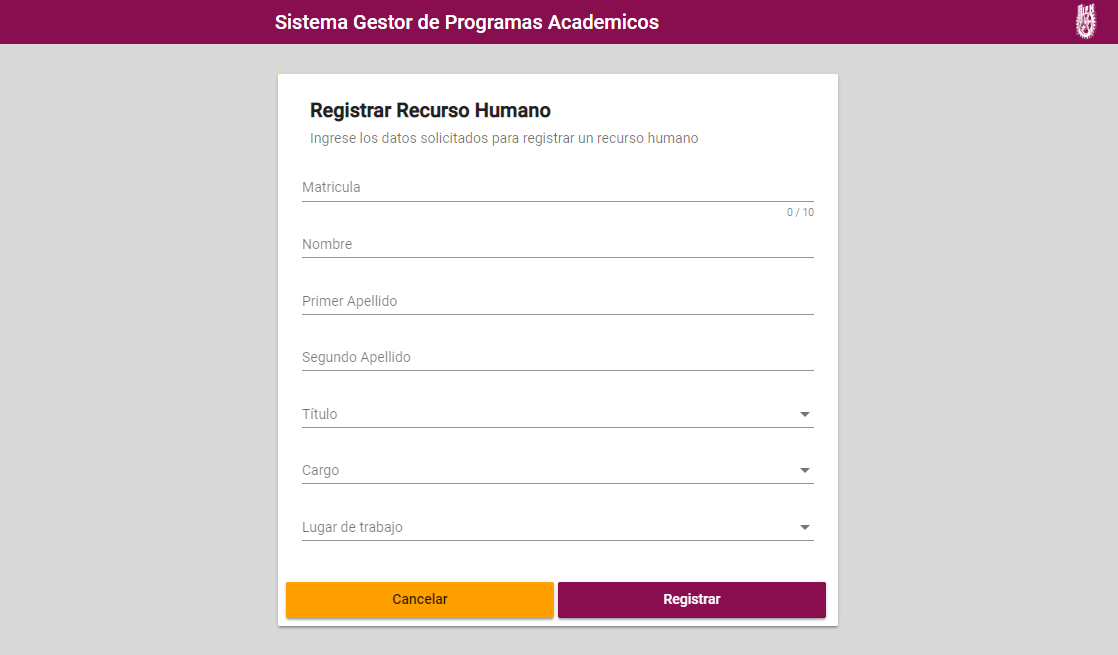
\includegraphics[width=0.7\linewidth]{images/SP1/RegistrarRH}}
            \caption{Pantalla para registrar Recursos Humanos}
            \label{registrarrh}
        \end{figure}
        
        En donde tendrá que ingresar los campos del nuevo Recurso Humano en el formulario. Un ejemplo del llenado sería el siguiente:
    
        \begin{figure}[!hbtp]
        	\centering
        	\hypertarget{ejreg}{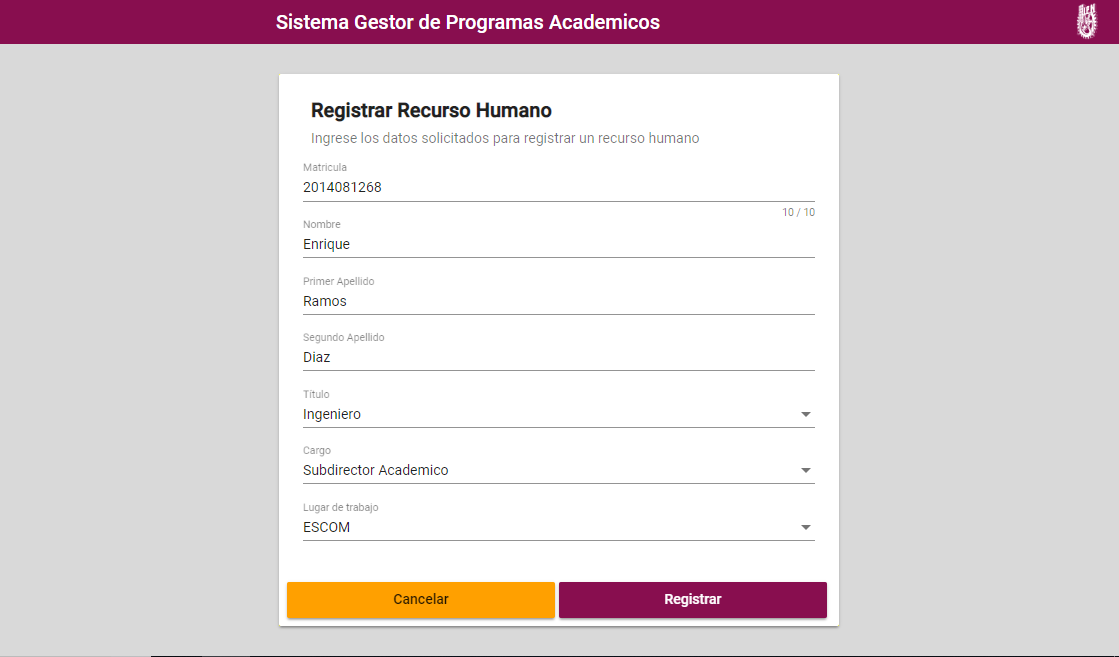
\includegraphics[width=0.7\linewidth]{images/SP1/Llenado}}
        	\caption{Ejemplo de llenado para agregar un nuevo Recurso Humano}
        	\label{ejreg}
        \end{figure}
        \newpage
        Si el Jefe de Innovación Educativa da clic en el botón \IUbutton{Cancelar} sin haber concluido el registro del Recurso Humano:

        \begin{figure}[!hbtp]
        	\centering
        	\hypertarget{cancel1}{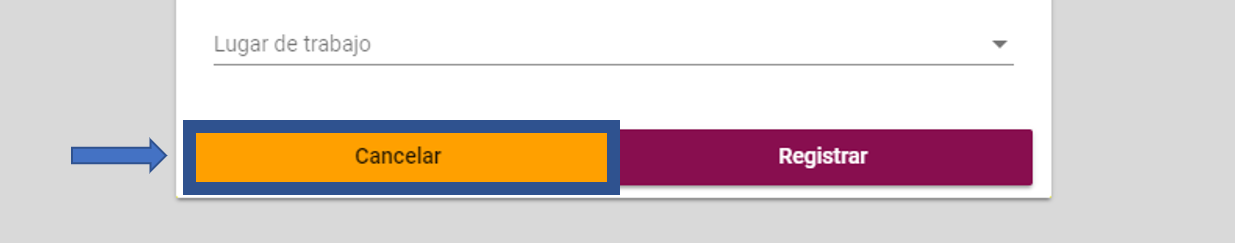
\includegraphics[width=0.7\linewidth]{images/SP1/BtnCancelar1}}
        	\caption{Botón ''Cancelar''}
        	\label{cancel1}
        \end{figure}

        El sistema mostrará el siguiente mensaje:
        \begin{figure}[!hbtp]
                \centering
                \hypertarget{buscar}{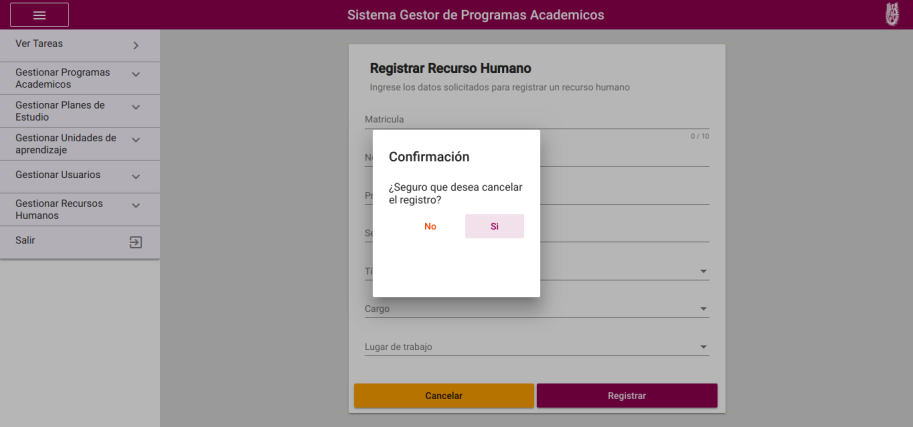
\includegraphics[width=0.7\linewidth]{images/SP1/MSG6}}
                \caption{MSG6. ¿Seguro que desea cancelar el registro?}
                \label{buscar}
        \end{figure}
        
        Para confirmar, el usuario debe dar clic en el botón \IUbutton{Sí}, y el Recurso Humano no será registrado.\\
        
        Para cancelar, el usuario debe dar clic en botón \IUbutton{No}, el mensaje se cerrará y continuaremos en el formulario. Aqui el Jefe de Innovación Educativa puede terminar el registro.\\
        
        A continuación, una vez verificados los datos, deberá de dar clic en el botón \IUbutton{Registrar}.
        \begin{figure}[!hbtp]
        	\centering
        	\hypertarget{btnreg}{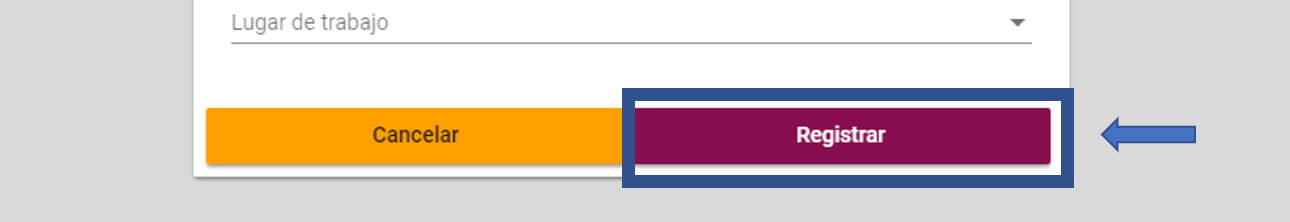
\includegraphics[width=0.7\linewidth]{images/SP1/BtnRegistrar}}
        	\caption{Botón ''Registrar''}
        	\label{btnreg}
        \end{figure}

        Si no hubieron errores, el sistema muestra el siguiente mensaje:
        \newpage
        \begin{figure}[!hbtp]
                \centering
                \hypertarget{buscar}{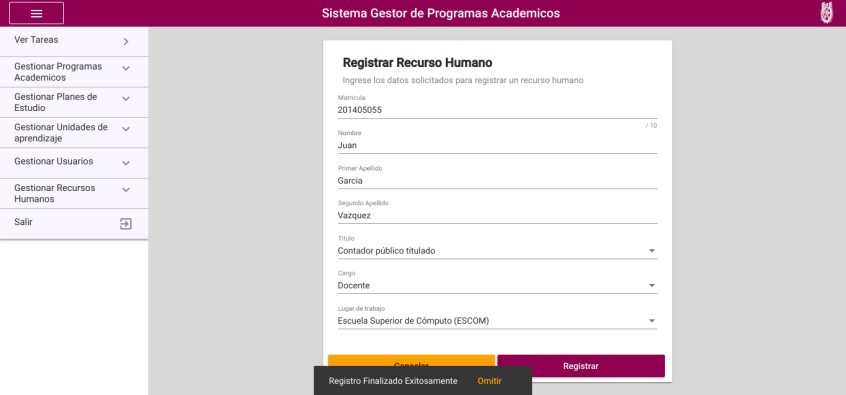
\includegraphics[width=0.7\linewidth]{images/SP1/MSG5}}
                \caption{MGS5. Registro finalizado exitosamente.}
                \label{buscar}
        \end{figure}

        Al dar clic en en botón \IUbutton{Aceptar}, el sistema redireccionará al usuario a la pantalla de \hyperlink{consultarrh}{\textit{Consultar Recursos Humanos}}, en donde podrá ver el nuevo Recurso Humano agregado.\\

        \subsection{Posibles errores}
            \begin{itemize}
            
            	\item Problemas con la conexión o el sistema
                
                	Si al momento de acceder a la pantalla de \hyperlink{registrarrh}{\textit{Registrar Recurso Humano}} o al intentar registrar un Recurso Humano, aparece alguno de los siguientes mensajes:
                	%Imagen MSG7 Y MSG25
                
                	Significa que existió un error de conexión o del sistema. Al dar clic en el botón \IUbutton{Aceptar}, el sistema redireccionará al usuario a la pantalla de \hyperlink{consultarrh}{\textit{Consultar Recursos Humanos}}. Debe esperar a que la página este disponible o intentar acceder nuevamente.
                
            	\item Campos vacíos al momento de agregar un nuevo Recurso Humano
            
                	Si el Jefe de Innovación Educativa dejo en blanco algún campo del formulario, y posteriormente dio clic en el botón \IUbutton{Registrar}, el sistema mostrará el siguiente mensaje:
                	%Imagen MSG32
                
                	Al dar clic en el botón \IUbutton{Aceptar}, el mensaje se cerrará y regresaremos al formulario, en donde el usuario deberá llenar el o los campos que dejo vacío. Si se continúan dejando campos en blanco y dando clic en el botón \IUbutton{Registrar}, aparecerá nuevamente el mensaje, hasta que todos los campos sean llenados.\\
                
                	También puede que no se haya seleccionado alguna opción en los campos: Título, Cargo o Lugar de Trabajo, verifique que exista un elemento seleccionado.
                
            	\item La matrícula ingresada ya existe
            
                	Si al momento de dar clic en el botón \IUbutton{Registrar} aparece el siguiente mensaje:
                	%Imagen MSG33
            
                	Significa que el Recurso Humano ya se encuentra registrado en el mensaje, por lo que éste impide que se vuelva a agregar nuevamente. Al dar clic en el botón \IUbutton{Aceptar}, el mensaje se cerrará y regresaremos al formulario. Aqui el Jefe de Innovación Educativa puede hacer dos acciones: verificar que la matrícula sea una no registrada previamente e intentar agregar al Recurso Humano nuevamente, o abandonar la pantalla de \hyperlink{registrarrh}{\textit{Registrar Recurso Humano}} e ir a otras partes del sistema.
            
            	\item Los campos ingresados no son válidos
    
                	Si al momento de dar clic en el botón \IUbutton{Registrar} aparece el siguiente mensaje:
            	    %Imagen MSG20
            
                	Significa que la composición de los datos ingresados en el formulario no es la correcta. Tenga en cuenta lo siguiente:
            
                	\begin{itemize}
                		\item La matrícula se compone de únicamente 10 caracteres númericos.
                		\item El nombre y apellidos debe iniciar con mayúscula.
                	\end{itemize}
            
            \end{itemize}
%-------------------------------------------------------------------------------------------------------
%-----------------------------EDICION DE RECURSOS HUMANOS--------------------------------
%-------------------------------------------------------------------------------------------------------

\newpage
    \section{Edición de Recursos Humanos}
        Si el Jefe de Innovación Educativa en la pantalla de \hyperlink{consultarrh}{\textit{Consultar Recursos Humanos}} dio clic en el botón con el icono de un lápiz amarillo de un Recurso Humano, aparece la siguiente pantalla:
        
        \begin{figure}[!hbtp]
        	\centering
        	\hypertarget{editarrh}{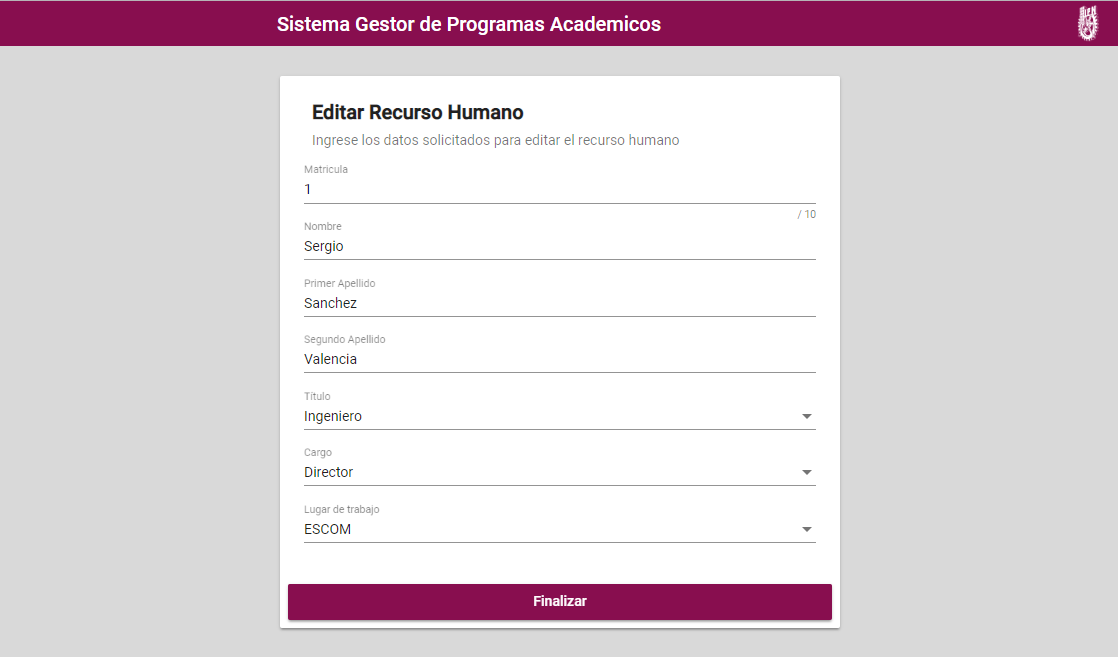
\includegraphics[width=0.7\linewidth]{images/SP1/EditarRH}}
        	\caption{Pantalla para la edición de Recursos Humanos}
        	\label{editarrh}
        \end{figure}

        En donde se cargaran los datos del Recurso Humano seleccionado en la pantalla de \hyperlink{consultarrh}{\textit{Consultar Recursos Humanos}} y llenará el formulario.\\
        
        A continuación, el usuario puede modificar todos los campos del Recurso Humano, a excepción de la matrícula:
        \begin{figure}[!hbtp]
        	\centering
        	\hypertarget{modif}{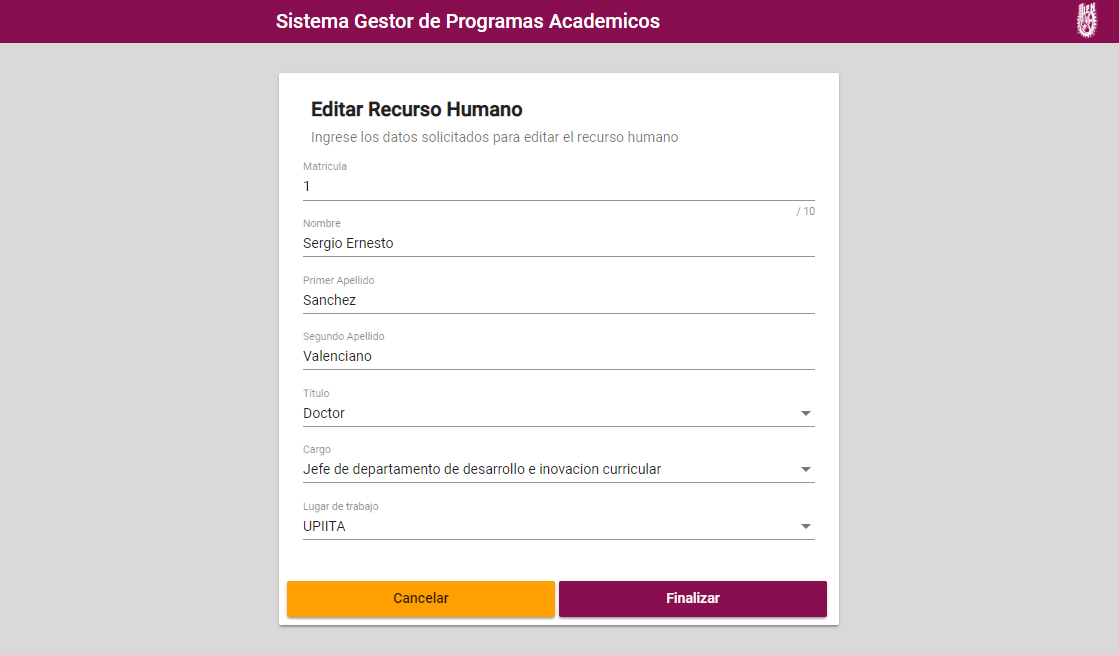
\includegraphics[width=0.7\linewidth]{images/SP1/Editado}}
        	\caption{Datos del Recurso Humano modificados}
        	\label{modif}
        \end{figure}

        Si el Jefe de Innovación Educativa da clic en el botón \IUbutton{Cancelar} sin haber concluido la edición del Recurso Humano:
        
        \begin{figure}[!hbtp]
        	\centering
        	\hypertarget{cancel2}{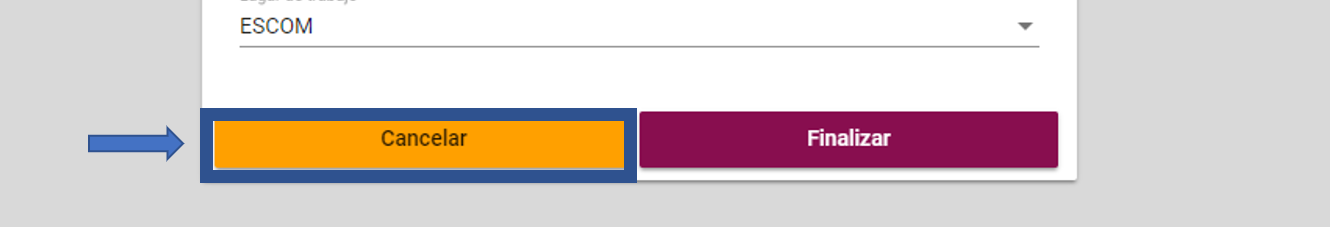
\includegraphics[width=0.7\linewidth]{images/SP1/BtnCancelar2}}
        	\caption{Botón ''Cancelar''}
        	\label{cancel2}
        \end{figure}
        
        El sistema mostrará el siguiente mensaje:
        %Imagen MSG30
        
        Para confirmar, el usuario debe dar clic en el botón \IUbutton{Sí}, y el Recurso Humano no será modificado.\\
        
        Para cancelar, el usuario debe dar clic en botón \IUbutton{No}, el mensaje se cerrará y continuaremos en el formulario. Aqui el Jefe de Innovación Educativa puede terminar la edición del Recurso Humano.\\

        Una vez verificados los datos, deberá de dar clic en el botón \IUbutton{Finalizar}.
        \begin{figure}[!hbtp]
        	\centering
        	\hypertarget{btnfin}{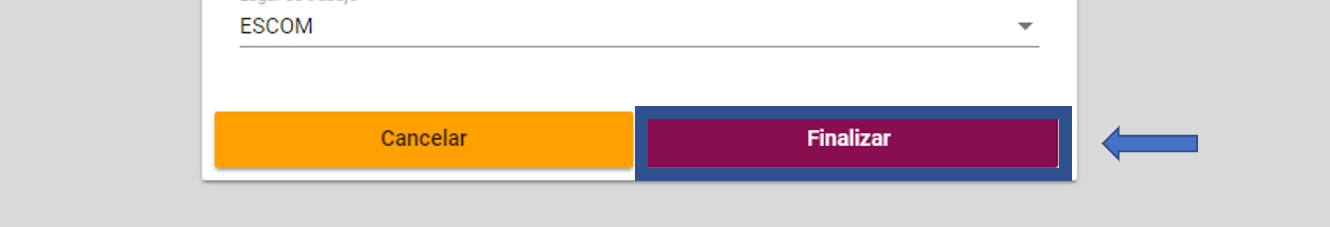
\includegraphics[width=0.7\linewidth]{images/SP1/BtnFinalizar}}
        	\caption{Botón ''Finalizar''}
        	\label{btnfin}
        \end{figure}
        
        Si no hubieron errores, el sistema muestra el siguiente mensaje:
        %Imagen MSG27
        
        Al dar clic en el botón \IUbutton{Aceptar}, el sistema redireccionará al usuario a la pantalla de \hyperlink{consultarrh}{\textit{Consultar Recursos Humanos}}, en donde podrá ver las modificaciones del Recurso Humano.\\
        
        \subsection{Posibles errores}
    
            \begin{itemize}
            	\item Problemas con la conexión o el sistema
            
                	Si al momento de acceder a la pantalla de \hyperlink{editarrh}{\textit{Editar Recurso Humano}} o al intentar modificar un Recurso Humano, aparece alguno de los siguientes mensajes:
            	    
            	    % Imagen MSG7 Y MSG25
            
                	Significa que existió un error de conexión o del sistema. Al dar clic en el botón \IUbutton{Aceptar}, el sistema redireccionará al usuario a la pantalla de \hyperlink{consultarrh}{\textit{Consultar Recursos Humanos}}. Debe esperar a que la página este disponible o intentar acceder nuevamente.
            
            	\item Campos vacíos al momento de modificar el Recurso Humano
            
                	Si el Jefe de Innovación Educativa dejo en blanco algún campo del formulario, y posteriormente dio clic en el botón \IUbutton{Finalizar}, el sistema mostrará el siguiente mensaje:
            	    
            	    % Imagen MSG32
            
            	    Al dar clic en botón \IUbutton{Aceptar}, el mensaje se cerrará y regresaremos al formulario, en donde el usuario deberá llenar el o los campos que dejo vacío. Si se continúan dejando campos en blanco y dando clic en el botón \IUbutton{Finalizar}, aparecerá nuevamente el mensaje, hasta que todos los campos sean llenados.
            
            	\item Los campos ingresados no son válidos
            
                	Si al momento de dar clic en el botón \IUbutton{Registrar} aparece el siguiente mensaje:
            	    % Imagen MSG20
            
                	Significa que la composición de los datos ingresados en el formulario no es la correcta, verifíquelos e intente de nuevo.
            
            \end{itemize}
